%%%%%%%%%%%%%%%%%%%%

% Project Name:
% File: main.tex
% Author: Keng-Yu Chen

%%%%%%%%%%%%%%%%%%%%

%%%%%%%%%%%%%%%%%%%%

% Project Name:
% File: header.tex
% Author: Keng-Yu Chen

%%%%%%%%%%%%%%%%%%%%

\documentclass[a4paper]{article}
\usepackage[a4paper, total={6in, 10in}]{geometry}
% \usepackage{showframe}
\usepackage{mathrsfs}
\usepackage{color}
\usepackage[utf8]{inputenc}
\usepackage[T1]{fontenc}
\usepackage{amsthm,amsmath,amssymb}
\usepackage{bm}
\usepackage{dsfont}
\usepackage{stmaryrd}
\usepackage{graphicx}
\usepackage{multicol}
\usepackage{multirow}
\usepackage{booktabs}
\usepackage{makecell}
\usepackage{wrapfig}
\usepackage{subcaption}
\usepackage{thmtools}
\usepackage{fancyhdr}
\usepackage[colorlinks=true, linkcolor=blue, citecolor=blue, urlcolor=blue]{hyperref}
\renewcommand\UrlFont{\color{blue}\rmfamily}

\usepackage{algorithm}
\usepackage{algpseudocode}
\renewcommand{\algorithmicrequire}{\textbf{Input:}}
\renewcommand{\algorithmicensure}{\textbf{Output:}}

\usepackage[
    lambda,
    advantage,
    operators,
    sets,
    adversary,
    landau,
    probability,
    notions,
    logic,
    ff,
    mm,
    primitives,
    events,
    complexity,
    oracles,
    asymptotics,
    keys
]{cryptocode}

% Set Self-defined Words
\renewcommand{\verify}{\mathsf{Vrfy}}
\newcommand{\Adv}{\mathbf{Adv}}
\newcommand{\R}{\mathbb{R}}
\newcommand{\N}{\mathbb{N}}
\newcommand{\Z}{\mathbb{Z}}
\newcommand{\Q}{\mathbb{Q}}

\makeatletter
\newcommand{\vast}{\bBigg@{4}}
\newcommand{\Vast}{\bBigg@{5}}
\makeatother

% Convert block[name] into a theorem-like format
\newtheorem{theorem}{Theorem}
\newtheorem{lemma}{Lemma}

\theoremstyle{definition}
\newtheorem{definition}{Definition}
\theoremstyle{definition}
\newtheorem{assumption}{Assumption}

\theoremstyle{plain}
\newtheorem{corollary}{Corollary}

\theoremstyle{remark}
\newtheorem{remark}{Remark}

% Add Referemces
\usepackage[
	backend=biber,
	style=alphabetic,
	sorting=ynt
]{biblatex}
\addbibresource{abbrev0.bib}
\addbibresource{reference.bib}

\title{\textbf{Finding a Close Point in a Lattice}}
\author{Keng-Yu Chen}
\date{\today}


\begin{document}
\maketitle

\begin{center}
	\fbox{\parbox{0.92\textwidth}{
		\textbf{Note:} This document was auto-generated by AI from a Markdown note on Notion.
		Its correctness has \emph{not} yet been verified — please check the reference papers and all definitions, algorithms, and proofs before relying on them.
	}}
\end{center}
\vspace{1em}

\section{Problem Setting}

The lattice $\mathcal{L}(\mathbf{B})$ of some matrix $\mathbf{B} = \{\mathbf{b}_1, \dots, \mathbf{b}_n\}$, where the $\mathbf{b}_i$'s are column vectors, is
\[
	\mathcal{L}(\mathbf{B}) = \left\{ \mathbf{B}x = \sum_{i=1}^n x_i \mathbf{b}_i : x_i \in \Z \right\}.
\]
The goal is that, given some vector $\mathbf{c}$, find a vector $\mathbf{z} \in \mathcal{L}(\mathbf{B})$ which is close to $\mathbf{c}$, with closeness measured by Euclidean distance.

\section{Preliminaries}

\begin{definition}[Gram--Schmidt Orthogonalization]
	The Gram--Schmidt orthogonalization (GSO) of a full-rank matrix $\mathbf{B}$ is $\mathbf{\tilde B} = \{\mathbf{\tilde b}_1, \dots, \mathbf{\tilde b}_n\}$ where
	\[
		\mathbf{\tilde b}_i = \mathbf{b}_i - \sum_{j=1}^{i-1} \frac{\langle \mathbf{b}_i, \mathbf{\tilde b}_j \rangle}{\langle \mathbf{\tilde b}_j, \mathbf{\tilde b}_j \rangle} \mathbf{\tilde b}_j.
	\]
\end{definition}

We can write $\mathbf{B} = \mathbf{\tilde B U}$, or equivalently $\mathbf{B}^t = \mathbf{L \tilde B}^t$, for some upper-triangular matrix $\mathbf{U}$ or lower-triangular matrix $\mathbf{L}$ with $1$'s on their diagonals, where
\[
	\mathbf{U} =
	\begin{bmatrix}
		1 & \dfrac{\langle \mathbf{b}_2, \mathbf{\tilde b}_1 \rangle}{\langle \mathbf{\tilde b}_1, \mathbf{\tilde b}_1 \rangle} & \dfrac{\langle \mathbf{b}_3, \mathbf{\tilde b}_1 \rangle}{\langle \mathbf{\tilde b}_1, \mathbf{\tilde b}_1 \rangle} & \cdots & \dfrac{\langle \mathbf{b}_n, \mathbf{\tilde b}_1 \rangle}{\langle \mathbf{\tilde b}_1, \mathbf{\tilde b}_1 \rangle} \\
		0 & 1 & \dfrac{\langle \mathbf{b}_3, \mathbf{\tilde b}_2 \rangle}{\langle \mathbf{\tilde b}_2, \mathbf{\tilde b}_2 \rangle} & \cdots & \dfrac{\langle \mathbf{b}_n, \mathbf{\tilde b}_2 \rangle}{\langle \mathbf{\tilde b}_2, \mathbf{\tilde b}_2 \rangle} \\
		0 & 0 & 1 & \cdots & \vdots \\
		\vdots & \vdots & \vdots & \ddots & \vdots \\
		0 & 0 & \cdots & 0 & 1
	\end{bmatrix}.
\]

\begin{definition}[Gaussian Function]
	The Gaussian function in $n$ dimensions is
	\[
		\rho_{s,\mathbf{c}}(\mathbf{x}) = \exp\left( -\pi \frac{\|\mathbf{x} - \mathbf{c}\|^2}{s^2} \right).
	\]
	We may omit $\mathbf{c}$ when $\mathbf{c} = \mathbf{0}$.
\end{definition}

\begin{definition}[Discrete Gaussian Distribution]
	The discrete Gaussian distribution over a lattice $\Lambda$ is
	\[
		D_{\Lambda,s,\mathbf{c}}(\mathbf{x}) = \frac{\exp\left( -\pi \frac{\|\mathbf{x}-\mathbf{c}\|^2}{s^2} \right)}{\sum_{\mathbf{v} \in \Lambda} \exp\left( -\pi \frac{\|\mathbf{v}-\mathbf{c}\|^2}{s^2} \right)} = \frac{\rho_{s,\mathbf{c}}(\mathbf{x})}{\rho_{s,\mathbf{c}}(\Lambda)}.
	\]
\end{definition}

\section{Babai's Round-off Algorithm~\cite{Bab85}}

\begin{algorithm}[H]
	\caption{Babai's Round-off Algorithm}
	\label{alg:babai}
	\begin{algorithmic}[1]
		\Require Basis $\mathbf{B}$, target vector $\mathbf{c}$
		\Ensure Vector $\mathbf{z} \in \mathcal{L}(\mathbf{B})$ close to $\mathbf{c}$
		\State Compute $\mathbf{B}^{-1}$
		\State $\mathbf{v} \gets \mathbf{B} \cdot \lfloor \mathbf{B}^{-1}\mathbf{c} \rceil$
		\State \Return $\mathbf{v}$
	\end{algorithmic}
\end{algorithm}

Note that
\[
	\mathbf{c} - \mathbf{v} = \mathbf{B} \cdot \mathbf{B}^{-1}\mathbf{c} - \mathbf{B} \cdot \lfloor \mathbf{B}^{-1}\mathbf{c} \rceil \in \mathbf{B} \cdot [-1,1]^n.
\]

\section{Nearest-Plane Algorithm~\cite{Kle00}}

\begin{algorithm}[H]
	\caption{Nearest-Plane Algorithm}
	\label{alg:nearest-plane}
	\begin{algorithmic}[1]
		\Require Basis $\mathbf{B}$, target vector $\mathbf{c}$
		\Ensure Vector $\mathbf{v}_0 \in \mathcal{L}(\mathbf{B})$ close to $\mathbf{c}$
		\State $\mathbf{c}_n \gets \mathbf{c}, \ \mathbf{v}_n \gets \mathbf{0}$
		\For{$i = n, \dots, 1$}
			\State $c_i' \gets \dfrac{\langle \mathbf{c}_i, \mathbf{\tilde b}_i \rangle}{\langle \mathbf{\tilde b}_i, \mathbf{\tilde b}_i \rangle}$
			\State $z_i \gets \lfloor c_i' \rceil$
			\State $\mathbf{c}_{i-1} \gets \mathbf{c}_i - z_i \mathbf{b}_i, \quad \mathbf{v}_{i-1} \gets \mathbf{v}_i + z_i \mathbf{b}_i$
		\EndFor
		\State \Return $\mathbf{v}_0$
	\end{algorithmic}
\end{algorithm}

\begin{figure}[htp]
	\centering
	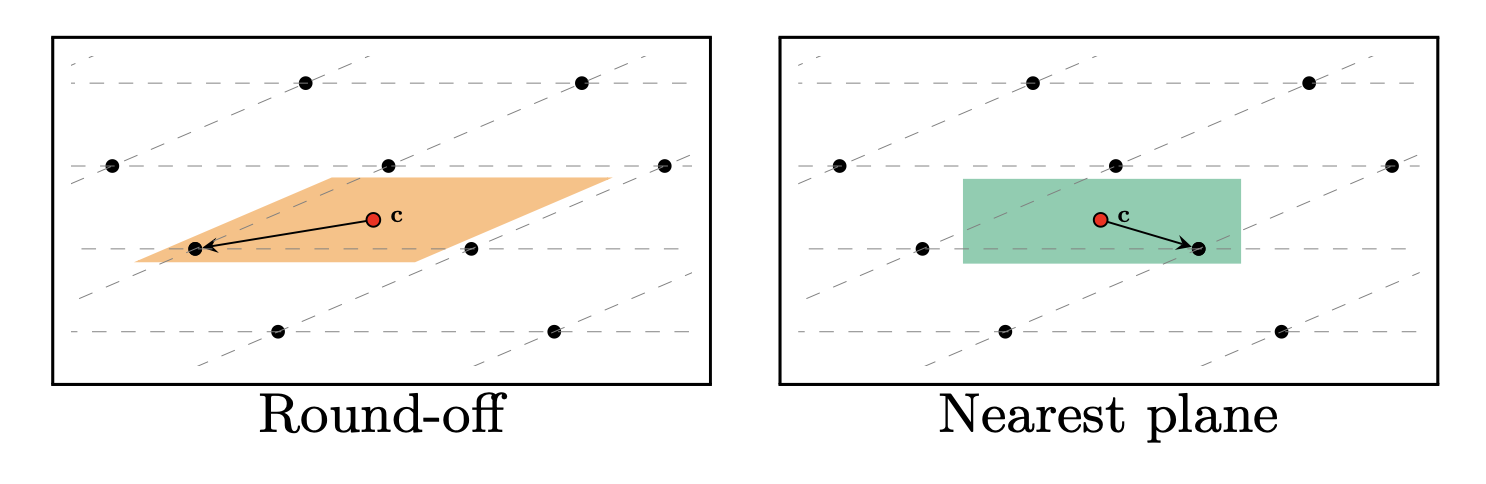
\includegraphics[width=0.8\textwidth]{Figure/illustration_from_DP16.png}
	\caption{Illustration of the nearest-plane algorithm, from~\cite{DP16}.}
	\label{fig:dp16-illustration}
\end{figure}


\begin{theorem}
	\label{thm:nearest-plane}
	\[
		\mathbf{v}_0 - \mathbf{c} = \sum_{i=1}^n (z_i - c_i') \mathbf{\tilde b}_i \in \mathbf{\tilde B} \cdot \left[-\frac{1}{2}, \frac{1}{2}\right]^n.
	\]
\end{theorem}

\begin{proof}
	We claim that for $j = 1, 2, \dots, n$,
	\[
		\mathbf{v}_0 - \mathbf{v}_j - \pi_j(\mathbf{c}_j) = \sum_{i=1}^j (z_i - c_i') \mathbf{\tilde b}_i,
	\]
	where $\pi_j(\cdot)$ is the orthogonal projection onto $\mathrm{span}(\mathbf{b}_1, \dots, \mathbf{b}_j)$,
	\[
		\pi_j(\mathbf{t}) = \sum_{k=1}^j \frac{\langle \mathbf{t}, \mathbf{\tilde b}_k \rangle}{\langle \mathbf{\tilde b}_k, \mathbf{\tilde b}_k \rangle} \mathbf{\tilde b}_k, \qquad \mathbf{\tilde b}_j = \mathbf{b}_j - \pi_{j-1}(\mathbf{b}_j).
	\]
	Observe that
	\[
		\pi_j(\mathbf{c}_j) = c_j' \mathbf{\tilde b}_j + \pi_{j-1}(\mathbf{c}_j), \qquad \mathbf{\tilde b}_j = \mathbf{b}_j - \pi_{j-1}(\mathbf{b}_j).
	\]
	Note that when $j = n$, the above equation becomes what we desire, since $\mathbf{v}_n = \mathbf{0}$ and $\pi_n(\mathbf{c}_n) = \pi_n(\mathbf{c}) = \mathbf{c}$.
	We prove this by induction. For $j = 1$,
	\[
		\mathbf{v}_0 - \mathbf{v}_1 - \pi_1(\mathbf{c}_1) = z_1 \mathbf{b}_1 - \pi_1(\mathbf{c}_1) = z_1 \mathbf{\tilde b}_1 - c_1' \mathbf{\tilde b}_1.
	\]
	Now suppose the equation holds for all $j < k$. For $j = k$,
	\begin{align*}
		\mathbf{v}_0 - \mathbf{v}_j - \pi_j(\mathbf{c}_j)
		&= \mathbf{v}_0 - (\mathbf{v}_{k-1} - z_k \mathbf{b}_k) - \pi_{k-1}(\mathbf{c}_k) + c_k' \mathbf{\tilde b}_k \\
		&= \mathbf{v}_0 - \mathbf{v}_{k-1} + z_k \mathbf{b}_k - \pi_{k-1}(\mathbf{c}_{k-1} + z_k \mathbf{b}_k) - c_k' \mathbf{\tilde b}_k \\
		&= \mathbf{v}_0 - \mathbf{v}_{k-1} - \pi_{k-1}(\mathbf{c}_{k-1}) + z_k (\mathbf{b}_k - \pi_{k-1}(\mathbf{b}_k)) - c_k' \mathbf{\tilde b}_k \\
		&= \sum_{i=1}^{k-1} (z_i - c_i') \mathbf{\tilde b}_i + z_k \mathbf{\tilde b}_k - c_k' \mathbf{\tilde b}_k.
	\end{align*}
\end{proof}

\subsection{Another Version via \texorpdfstring{$\mathbf{U}$}{U}}

\begin{algorithm}[H]
	\caption{Nearest-Plane Algorithm (via $\mathbf{U}$)}
	\label{alg:nearest-plane-u}
	\begin{algorithmic}[1]
		\Require Basis $\mathbf{B}$, target vector $\mathbf{c}$
		\Ensure Vector $\mathbf{v} \in \mathcal{L}(\mathbf{B})$ close to $\mathbf{c}$
		\State Find $\mathbf{t} = \mathbf{B}^{-1}\mathbf{c}$ such that $\mathbf{B}\mathbf{t} = \mathbf{c}$
		\For{$i = n, \dots, 1$}
			\State $t_i' \gets t_i + \sum_{j > i} \mathbf{U}_{ij} (t_j - z_j)$
			\State $z_i \gets \lfloor t_i' \rceil$
		\EndFor
		\State \Return $\mathbf{v} = \sum_{i=1}^n z_i \mathbf{b}_i$
	\end{algorithmic}
\end{algorithm}

\begin{proof}[Proof of Equivalence]
	Algorithms \ref{alg:nearest-plane} and \ref{alg:nearest-plane-u} compute the same thing. We show that $t_i' = c_i'$. Note that
	\[
		c_i' = \frac{\langle \mathbf{c} - \sum_{j>i} z_j \mathbf{b}_j, \mathbf{\tilde b}_i \rangle}{\langle \mathbf{\tilde b}_i, \mathbf{\tilde b}_i \rangle} = \frac{\langle \mathbf{c}, \mathbf{\tilde b}_i \rangle}{\langle \mathbf{\tilde b}_i, \mathbf{\tilde b}_i \rangle} - \frac{\langle \sum_{j>i} z_j \mathbf{b}_j, \mathbf{\tilde b}_i \rangle}{\langle \mathbf{\tilde b}_i, \mathbf{\tilde b}_i \rangle}.
	\]
	Also, $\mathbf{U}_{ij} = \dfrac{\langle \mathbf{b}_j, \mathbf{\tilde b}_i \rangle}{\langle \mathbf{\tilde b}_i, \mathbf{\tilde b}_i \rangle}$, so
	\[
		\sum_{j>i} \mathbf{U}_{ij} z_j = \sum_{j>i} z_j \frac{\langle \mathbf{b}_j, \mathbf{\tilde b}_i \rangle}{\langle \mathbf{\tilde b}_i, \mathbf{\tilde b}_i \rangle} = \frac{\langle \sum_{j>i} z_j \mathbf{b}_j, \mathbf{\tilde b}_i \rangle}{\langle \mathbf{\tilde b}_i, \mathbf{\tilde b}_i \rangle}.
	\]
	It remains to show that $t_i + \sum_{j>i} \mathbf{U}_{ij} t_j = \dfrac{\langle \mathbf{c}, \mathbf{\tilde b}_i \rangle}{\langle \mathbf{\tilde b}_i, \mathbf{\tilde b}_i \rangle}$. Since $\mathbf{\tilde B}$ is full-rank and orthogonal,
	\[
		\mathbf{c} = \sum_{i=1}^n \frac{\langle \mathbf{c}, \mathbf{\tilde b}_i \rangle}{\langle \mathbf{\tilde b}_i, \mathbf{\tilde b}_i \rangle} \mathbf{\tilde b}_i = \mathbf{\tilde B} \left[ \frac{\langle \mathbf{c}, \mathbf{\tilde b}_i \rangle}{\langle \mathbf{\tilde b}_i, \mathbf{\tilde b}_i \rangle} \right]_i.
	\]
	Therefore,
	\[
		\left[ \frac{\langle \mathbf{c}, \mathbf{\tilde b}_i \rangle}{\langle \mathbf{\tilde b}_i, \mathbf{\tilde b}_i \rangle} \right]_i = \mathbf{\tilde B}^{-1} \mathbf{c} = \mathbf{\tilde B}^{-1} \mathbf{B} \mathbf{t} = \mathbf{U}\mathbf{t} = \left[ \sum_{j=1}^n \mathbf{U}_{ij} t_j \right]_i = \left[ t_i + \sum_{j>i} \mathbf{U}_{ij} t_j \right]_i.
	\]
\end{proof}

\begin{corollary}[Equivalent Formulation of Theorem~\ref{thm:nearest-plane}]
	\label{cor:thm1-alt}
	Let $\mathbf{t}' = (t_1', \dots, t_n')$. Then
	\[
		\mathbf{B}(\mathbf{z} - \mathbf{t}) = \mathbf{\tilde B}(\mathbf{z} - \mathbf{t}') \in \mathbf{\tilde B} \cdot \left[-\frac{1}{2}, \frac{1}{2}\right]^n.
	\]
\end{corollary}

\begin{proof}
	\begin{align*}
		\mathbf{\tilde B}(\mathbf{z} - \mathbf{t}')
		&= \sum_{i=1}^n (z_i - t_i') \mathbf{\tilde b}_i \\
		&= \sum_{i=1}^n \left( z_i - t_i - \sum_{j>i} \mathbf{U}_{ij} (t_j - z_j) \right) \mathbf{\tilde b}_i \\
		&= \sum_{i=1}^n \left( \sum_{j \geq i} \mathbf{U}_{ij} (z_j - t_j) \right) \mathbf{\tilde b}_i \\
		&= \sum_{j=1}^n (z_j - t_j) \sum_{i < j} \mathbf{U}_{ij} \mathbf{\tilde b}_i \\
		&= \sum_{j=1}^n (z_j - t_j) \mathbf{b}_j \\
		&= \mathbf{B}(\mathbf{z} - \mathbf{t}).
	\end{align*}
\end{proof}

\section{Randomized Version~\cite{GPV08}}

\begin{algorithm}[H]
	\caption{Randomized Nearest-Plane (Discrete Gaussian Sampler)}
	\label{alg:randomized-gpv}
	\begin{algorithmic}[1]
		\Require Basis $\mathbf{B}$, target vector $\mathbf{c}$, parameter $\sigma$
		\Ensure Vector $\mathbf{v}_0 \in \mathcal{L}(\mathbf{B})$ distributed as $D_{\mathcal{L}(\mathbf{B}), \sigma, \mathbf{c}}$
		\State $\mathbf{c}_n \gets \mathbf{c}, \ \mathbf{v}_n \gets \mathbf{0}$
		\For{$i = n, \dots, 1$}
			\State $c_i' \gets \dfrac{\langle \mathbf{c}_i, \mathbf{\tilde b}_i \rangle}{\langle \mathbf{\tilde b}_i, \mathbf{\tilde b}_i \rangle}, \quad \sigma_i \gets \dfrac{\sigma}{\|\mathbf{\tilde b}_i\|}$
			\State $z_i \gets D_{\Z, \sigma_i, c_i'}$
			\State $\mathbf{c}_{i-1} \gets \mathbf{c}_i - z_i \mathbf{b}_i, \quad \mathbf{v}_{i-1} \gets \mathbf{v}_i + z_i \mathbf{b}_i$
		\EndFor
		\State \Return $\mathbf{v}_0$
	\end{algorithmic}
\end{algorithm}

\begin{algorithm}[H]
	\caption{Randomized Nearest-Plane via $\mathbf{U}$}
	\label{alg:randomized-gpv-u}
	\begin{algorithmic}[1]
		\Require Basis $\mathbf{B}$, target vector $\mathbf{c}$, parameter $\sigma$
		\Ensure Vector $\mathbf{v} \in \mathcal{L}(\mathbf{B})$ distributed as $D_{\mathcal{L}(\mathbf{B}), \sigma, \mathbf{c}}$
		\State Find $\mathbf{t} = \mathbf{B}^{-1}\mathbf{c}$ such that $\mathbf{B}\mathbf{t} = \mathbf{c}$
		\For{$i = n, \dots, 1$}
			\State $t_i' \gets t_i + \sum_{j > i} \mathbf{U}_{ij} (t_j - z_j)$
			\State $\sigma_i \gets \dfrac{\sigma}{\|\mathbf{\tilde b}_i\|}$
			\State $z_i \gets D_{\Z, \sigma_i, t_i'}$
		\EndFor
		\State \Return $\mathbf{v} = \sum_{i=1}^n z_i \mathbf{b}_i$
	\end{algorithmic}
\end{algorithm}

Note that Theorem~\ref{thm:nearest-plane} also holds for the randomized algorithms above.

\begin{theorem}[{Lemma 4.5 in~\cite{GPV08}}]
	\label{thm:gpv-density}
	For $\sigma \geq \|\mathbf{\tilde B}\| \cdot \omega(\sqrt{\log n}) = \max_i \|\mathbf{\tilde b}_i\| \cdot \omega(\sqrt{\log n})$,
	\[
		\mathbf{v}_0 \stackrel{\Delta}{\sim} D_{\mathcal{L}(\mathbf{B}), \sigma, \mathbf{c}}.
	\]
	Concretely, we require $\sigma \geq \|\mathbf{\tilde B}\| \cdot \eta_\epsilon(\Z)$, which ensures $\sigma_i \geq \eta_\epsilon(\Z)$ for all $i$.
\end{theorem}

\begin{proof}
	Let $\mathbf{v}_0 = \sum_{i=1}^n z_i \mathbf{b}_i$ where $z_i \gets D_{\Z, \sigma_i', c_i'}$. The probability of outputting $\mathbf{v}_0$ is
	\[
		\prod_{i=1}^n D_{\Z, \sigma_i', c_i'}(z_i) = \frac{\prod \rho_{\sigma_i', c_i'}(z_i)}{\prod \rho_{\sigma_i', c_i'}(\Z)}.
	\]
	Note that $\rho_{\sigma_i', c_i'}(x) = \rho_{\sigma_i'}(x - c_i') = \rho_\sigma((x-c_i') \cdot \|\mathbf{\tilde b}_i\|)$. The numerator equals
	\[
		\prod_{i=1}^n \rho_{\sigma_i', c_i'}(z_i) = \prod_{i=1}^n \rho_\sigma((z_i - c_i') \cdot \|\mathbf{\tilde b}_i\|) = \rho_\sigma\left( \sum_{i=1}^n (z_i - c_i') \cdot \mathbf{\tilde b}_i \right) = \rho_\sigma(\mathbf{v}_0 - \mathbf{c}) = \rho_{\sigma, \mathbf{c}}(\mathbf{v}_0).
	\]
	Now we need the denominator to be close to $\rho_{\sigma, \mathbf{c}}(\mathcal{L}(\mathbf{B}))$. Recall the smoothing-parameter lemma: since $\sigma_i \geq \omega(\sqrt{\log n})$, $\sigma_i \geq \eta_\epsilon(\Z)$ for negligible $\epsilon(n)$, and
	\[
		\rho_{\sigma_i', c_i'}(\Z) \in \left[ \frac{1-\epsilon}{1+\epsilon}, 1 \right] \cdot \rho_{\sigma_i'}(\Z).
	\]
	Therefore,
	\[
		\prod \rho_{\sigma_i', c_i'}(\Z) \in \left[ \left(\frac{1-\epsilon}{1+\epsilon}\right)^n, 1 \right] \cdot \prod \rho_{\sigma_i'}(\Z).
	\]
	This range no longer depends on $c_i'$ or $\mathbf{c}$. In particular, the probability of outputting $\mathbf{v}_0$ equals
	\[
		\Pr[\mathbf{v}_0] = \frac{\rho_{\sigma, \mathbf{c}}(\mathbf{v}_0)}{\prod \rho_{\sigma_i', c_i'}(\Z)} \in \rho_{\sigma, \mathbf{c}}(\mathbf{v}_0) \cdot \left[ 1, \left(\frac{1+\epsilon}{1-\epsilon}\right)^n \right] \cdot \frac{1}{\prod \rho_{\sigma_i'}(\Z)}.
	\]
	Since summing over all possible $\mathbf{v}_0$ gives $1$,
	\[
		\prod \rho_{\sigma_i'}(\Z) \in \left[ 1, \left(\frac{1+\epsilon}{1-\epsilon}\right)^n \right] \cdot \rho_{\sigma, \mathbf{c}}(\mathcal{L}(\mathbf{B})).
	\]
	So the probability of outputting $\mathbf{v}_0$ is within $\left[ \left(\frac{1-\epsilon}{1+\epsilon}\right)^n, \left(\frac{1+\epsilon}{1-\epsilon}\right)^n \right]$ of $D_{\mathcal{L}(\mathbf{B}), \sigma, \mathbf{c}}(\mathbf{v}_0)$. For negligible $\epsilon$, $\left(\frac{1+\epsilon}{1-\epsilon}\right)^n$ is also negligible, so the statistical distance is negligible.

	Concretely, the statistical distance is smaller than
	\[
		\frac{1}{2} \left[ \left(\frac{1+\epsilon}{1-\epsilon}\right)^n - 1 \right] = \frac{1}{2} \epsilon'(\epsilon, n),
	\]
	where $\epsilon' \approx 2n\epsilon$. Letting the statistical distance $\frac{1}{2}\epsilon' = 2^{-\lambda}$ be fixed (for a given security parameter $\lambda$), the requirement on $\sigma$ becomes
	\[
		\sigma \geq \|\mathbf{\tilde B}\| \cdot \eta_{2^{-\lambda}}(\Z^n),
	\]
	because we require
	\[
		\sigma_i \geq \eta_\epsilon(\Z) \approx \eta_{n\epsilon}(\Z^n) \approx \eta_{\frac{1}{2}\epsilon'}(\Z^n) = \eta_{2^{-\lambda}}(\Z^n).
	\]
	This matches the theorem in~\cite{Pre17}.

\end{proof}

\begin{remark}
	This also implies that by calling this algorithm multiple times, one can obtain the ``closest'' point with high probability.
\end{remark}


\section{Fast Fourier Orthogonalization~\cite{DP16}}

In consistency with the paper, we use $\mathbf{B} = \mathbf{L\tilde B}$ for some orthogonal $\mathbf{\tilde B} = \{\mathbf{\tilde b}_1, \dots, \mathbf{\tilde b}_n\}$ and unit lower-triangular matrix $\mathbf{L}$, where the $\mathbf{\tilde b}_i$ are row vectors,
\[
	\mathbf{\tilde b}_i = \mathbf{b}_i - \sum_{j=1}^{i-1} \frac{\langle \mathbf{b}_i, \mathbf{\tilde b}_j \rangle}{\langle \mathbf{\tilde b}_j, \mathbf{\tilde b}_j \rangle} \mathbf{\tilde b}_j, \qquad
	\mathbf{L} =
	\begin{bmatrix}
		1 & 0 & 0 & \cdots & 0 \\
		\dfrac{\langle \mathbf{b}_2, \mathbf{\tilde b}_1 \rangle}{\langle \mathbf{\tilde b}_1, \mathbf{\tilde b}_1 \rangle} & 1 & 0 & \cdots & 0 \\
		\dfrac{\langle \mathbf{b}_3, \mathbf{\tilde b}_1 \rangle}{\langle \mathbf{\tilde b}_1, \mathbf{\tilde b}_1 \rangle} & \dfrac{\langle \mathbf{b}_3, \mathbf{\tilde b}_2 \rangle}{\langle \mathbf{\tilde b}_2, \mathbf{\tilde b}_2 \rangle} & 1 & \cdots & \vdots \\
		\vdots & \vdots & \vdots & \ddots & \vdots \\
		\dfrac{\langle \mathbf{b}_n, \mathbf{\tilde b}_1 \rangle}{\langle \mathbf{\tilde b}_1, \mathbf{\tilde b}_1 \rangle} & \dfrac{\langle \mathbf{b}_n, \mathbf{\tilde b}_2 \rangle}{\langle \mathbf{\tilde b}_2, \mathbf{\tilde b}_2 \rangle} & \cdots & 0 & 1
	\end{bmatrix}.
\]

\subsection{Definitions}

Let $R_d = \R[X]/(X^d - 1)$ for $d = 2^h$; we call this the circular convolution ring. Let $a = \sum_{i \in \Z_d} a_i X^i \in R_d$.

\begin{definition}[Adjoint]
	\[
		a^*(X) = a(1/X) \bmod (X^d - 1) = a_0 + \sum_{i=1}^{d-1} a_i X^{d-i}.
	\]
	Let $\Omega = \{\zeta \mid \zeta^d - 1 = 0\}$. Then $a^*$ is the unique element of $R_d$ such that $a^*(\zeta) = \overline{a(\zeta)}$ for all $\zeta \in \Omega$.
\end{definition}

\begin{definition}[Inner Product]
	\[
		\langle a, b \rangle = \sum_{\zeta^d - 1 = 0} a(\zeta) \cdot \overline{b(\zeta)}, \qquad \|a\| = \sqrt{\langle a, a \rangle}.
	\]
\end{definition}

This differs from the canonical inner product $\langle a, b \rangle_2 = \sum_i a_i b_i$. In fact, $\{a(\zeta)\}_{\zeta^d - 1 = 0} = [a_0, \dots, a_{d-1}] \mathbf{V}_d$, where $\mathbf{V}_d = (\zeta_d^{ij})_{i,j}$ is the Vandermonde matrix. Therefore, if $a, b \in R_d$ (hence real-coefficient),
\[
	\langle a, b \rangle = [a_0, \dots, a_{d-1}] \mathbf{V}_d \cdot \mathbf{V}_d^* \cdot [b_0, \dots, b_{d-1}] = d \cdot \langle a, b \rangle_2.
\]

\begin{definition}[Coefficient Maps]
	\leavevmode\par
	\begin{enumerate}
		\item The coefficient vector $c(a) = (a_0, \dots, a_{d-1})$.
		\item The circulant matrix
		\[
			C(a) = \begin{bmatrix}
				a_0 & a_1 & \dots & a_{d-1} \\
				a_{d-1} & a_0 & \dots & a_{d-2} \\
				\ddots & \ddots & \ddots & \ddots \\
				a_1 & a_2 & \dots & a_0
			\end{bmatrix}
			=
			\begin{bmatrix}
				c(a) \\ c(Xa) \\ \vdots \\ c(X^{d-1}a)
			\end{bmatrix}
			\in \R^{d \times d}.
		\]
		\item $C(a) C(b) = C(ab)$.
		\item $c(a) C(b) = c(ab)$.
		\item $C(a)^* = C(a^*)$.
	\end{enumerate}
\end{definition}

\subsection{LDL Decomposition \texorpdfstring{$\mathsf{LDL}_{R_d}(\mathbf{G})$}{LDL\_Rd(G)}}

Let $\mathbf{G} = \mathbf{BB}^*$. The LDL decomposition is $\mathbf{G} = \mathbf{LDL}^*$, where $\mathbf{D} = \tilde{\mathbf{B}}\tilde{\mathbf{B}}^*$ and $\mathbf{B} = \mathbf{L\tilde B}$.

\begin{algorithm}[H]
	\caption{$\mathsf{LDL}_{R_d}(\mathbf{G} \in R_d^{n \times n})$}
	\label{alg:ldl-rd}
	\begin{algorithmic}[1]
		\Require Gram matrix $\mathbf{G} \in R_d^{n \times n}$
		\Ensure Unit lower-triangular $\mathbf{L}$, diagonal $\mathbf{D}$ with $\mathbf{G} = \mathbf{LDL}^*$
		\State $\mathbf{L}, \mathbf{D} \gets \mathbf{0}^{n \times n}$
		\For{$i = 1$ to $n$}
			\State $L_{ii} \gets 1$
			\State $D_i \gets G_{ii} - \sum_{j < i} L_{ij} L_{ij}^* D_j$
			\For{$j = 1$ to $i-1$}
				\State $L_{ij} \gets \dfrac{1}{D_j} \left( G_{ij} - \sum_{k < j} L_{ik} L_{jk}^* D_k \right)$
			\EndFor
		\EndFor
		\State \Return $\mathbf{L}, \mathbf{D}$
	\end{algorithmic}
\end{algorithm}

\subsection{Nearest-Plane Algorithm \texorpdfstring{$\mathsf{NP}_\R(\mathbf{t}, \mathbf{L})$}{NP\_R(t,L)}}

We rewrite the nearest-plane algorithm in accordance with the notation above. Given a target vector $\mathbf{t}$ and $\mathbf{L}$ such that $\mathbf{B} = \mathbf{L\tilde B}$:

\begin{algorithm}[H]
	\caption{$\mathsf{NP}_\R(\mathbf{t}, \mathbf{L})$}
	\label{alg:np-r}
	\begin{algorithmic}[1]
		\Require Target vector $\mathbf{t}$, unit lower-triangular $\mathbf{L}$
		\Ensure $\mathbf{z} \in \Z^n$
		\For{$j = n, \dots, 1$}
			\State $t_j' \gets t_j + \sum_{i>j} (t_i - z_i) \mathbf{L}_{ij}$
			\State $z_j \gets \lfloor t_j' \rceil$
		\EndFor
		\State \Return $\mathbf{z} = (z_1, \dots, z_n)$
	\end{algorithmic}
\end{algorithm}

It is guaranteed that $(\mathbf{t} - \mathbf{z}) \mathbf{B} \in \left[-\frac{1}{2}, \frac{1}{2}\right]^n \cdot \tilde{\mathbf{B}}$.

\subsection{Linearization}

Let $d = 2^h$ and $d' = 2^{h'}$ for some $h' \leq h$, and let $k = d/d'$, $Y = X^k$.

\begin{definition}[$V_{d/d'} : R_d^m \to R_{d'}^{km}$]
	\leavevmode\par
	\begin{enumerate}
		\item For $d = d' = 1$, $V_{d/d'}$ is the identity.
		\item For $d' = \mathrm{gpd}(d) = 2^{h-1}$: given $a \in R_d$, write $a = \sum_{i \in \Z_k} X^i a_i(Y) = a_0(X^2) + X a_1(X^2)$ with $a_i \in R_{d'}$. Then $V_{d/d'}(a) = (a_0, \dots, a_{k-1})$.
		\item Extend $V_{d/d'}$ from $m=1$ to $m>1$ component-wise.
		\item For a tower of proper divisors $d'' \mid d' \mid d$ and any $a \in R_d$,
		\[
			V_{d/d''}(a) = V_{d'/d''} \circ V_{d/d'}(a) \in R_{d''}^{d/d''}.
		\]
	\end{enumerate}
\end{definition}

\begin{definition}[$M_{d/d'} : R_d^{n \times m} \to R_{d'}^{kn \times km}$]
	\leavevmode\par
	\begin{enumerate}
		\item For $d = d' = 1$, $M_{d/d'}$ is the identity.
		\item For $d' = 2^{h-1}$: given $a \in R_d$, write $a = \sum_{i \in \Z_k} X^i a_i(Y)$ with $a_i \in R_{d'}$, and set
		\[
			M_{d/d'}(a) =
			\begin{bmatrix}
				a_0 & a_1 & \dots & a_{k-1} \\
				Ya_{k-1} & a_0 & \dots & a_{k-2} \\
				\ddots & \ddots & \ddots & \ddots \\
				Ya_1 & Ya_2 & \dots & a_0
			\end{bmatrix}
			=
			\begin{bmatrix}
				V_{d/d'}(a) \\ V_{d/d'}(Ya) \\ \vdots \\ V_{d/d'}(Y^{d'-1}a)
			\end{bmatrix}
			=
			\begin{bmatrix}
				a_0 & a_1 \\ X^2 a_1 & a_0
			\end{bmatrix}.
		\]
		\item Extend $M_{d/d'}$ from $n=m=1$ to $n,m>1$ component-wise.
		\item For a tower of proper divisors $d'' \mid d' \mid d$ and any $a \in R_d$,
		\[
			M_{d/d''}(a) = M_{d'/d''} \circ M_{d/d'}(a) \in R_{d''}^{d/d'' \times d/d''}.
		\]
	\end{enumerate}
\end{definition}

\subsubsection{Example}

Let $c(a) = (0,1,2,3,4,5,6,7)$, so $a_0 = (0,2,4,6)$ and $a_1 = (1,3,5,7)$:
\[
	C(a) = \begin{bmatrix}
		0 & 1 & \dots & 7 \\
		7 & 0 & \dots & 6 \\
		\ddots & \ddots & \ddots & \ddots \\
		1 & 2 & \dots & 0
	\end{bmatrix}.
\]
Then $c(V_{8/4}(a)) = ((0,2,4,6),(1,3,5,7))$ and
\[
	M_{8/4}(a) = \begin{bmatrix}
		(0,2,4,6) & (1,3,5,7) \\
		X^2(1,3,5,7) & (0,2,4,6)
	\end{bmatrix}
	=
	\begin{bmatrix}
		(0,2,4,6) & (1,3,5,7) \\
		(7,1,3,5) & (0,2,4,6)
	\end{bmatrix},
\]
\[
	C(M_{8/4}(a)) = \begin{bmatrix}
		0 & 2 & 4 & 6 & 1 & 3 & 5 & 7 \\
		6 & 0 & 2 & 4 & 7 & 1 & 3 & 5 \\
		\ddots & \ddots & \ddots & \ddots & \ddots & \ddots & \ddots & \ddots \\
		7 & 1 & 3 & 5 & 0 & 2 & 4 & 6 \\
		5 & 7 & 1 & 3 & 6 & 0 & 2 & 4 \\
		\ddots & \ddots & \ddots & \ddots & \ddots & \ddots & \ddots & \ddots
	\end{bmatrix}.
\]
Similarly, $c(V_{8/2}(a)) = (((0,4),(2,6)),((1,5),(3,7)))$ and
\[
	M_{8/2}(a) =
	\begin{bmatrix}
		\begin{bmatrix} (0,4) & (2,6) \\ (6,2) & (0,4) \end{bmatrix} &
		\begin{bmatrix} (1,5) & (3,7) \\ (7,3) & (1,5) \end{bmatrix} \\[1em]
		\begin{bmatrix} (7,3) & (1,5) \\ (5,1) & (7,3) \end{bmatrix} &
		\begin{bmatrix} (0,4) & (2,6) \\ (6,2) & (0,4) \end{bmatrix}
	\end{bmatrix},
\]
\[
	M_{8/1}(a) = C(M_{8/2}(a)) =
	\begin{bmatrix}
		\begin{bmatrix} 0 & 4 \\ 4 & 0 \end{bmatrix} & \begin{bmatrix} 2 & 6 \\ 6 & 2 \end{bmatrix} & \begin{bmatrix} 1 & 5 \\ 5 & 1 \end{bmatrix} & \begin{bmatrix} 3 & 7 \\ 7 & 3 \end{bmatrix} \\[1em]
		\begin{bmatrix} 6 & 2 \\ 2 & 6 \end{bmatrix} & \begin{bmatrix} 0 & 4 \\ 4 & 0 \end{bmatrix} & \begin{bmatrix} 7 & 3 \\ 3 & 7 \end{bmatrix} & \begin{bmatrix} 1 & 5 \\ 5 & 1 \end{bmatrix} \\[1em]
		\begin{bmatrix} 7 & 3 \\ 3 & 7 \end{bmatrix} & \begin{bmatrix} 1 & 5 \\ 5 & 1 \end{bmatrix} & \begin{bmatrix} 0 & 4 \\ 4 & 0 \end{bmatrix} & \begin{bmatrix} 2 & 6 \\ 6 & 2 \end{bmatrix} \\[1em]
		\begin{bmatrix} 5 & 1 \\ 1 & 5 \end{bmatrix} & \begin{bmatrix} 7 & 3 \\ 3 & 7 \end{bmatrix} & \begin{bmatrix} 6 & 2 \\ 2 & 6 \end{bmatrix} & \begin{bmatrix} 0 & 4 \\ 4 & 0 \end{bmatrix}
	\end{bmatrix}.
\]

\subsubsection{Properties}

\begin{enumerate}
	\item $M_{d/d'}(\mathbf{A} \cdot \mathbf{B}) = M_{d/d'}(\mathbf{A}) M_{d/d'}(\mathbf{B})$.
	\item $V_{d/d'}(ab) = V_{d/d'}(a) \cdot M_{d/d'}(b)$.
	\item $\langle V(\mathbf{a}), V(\mathbf{b}) \rangle = \langle \mathbf{a}, \mathbf{b} \rangle_2$, the canonical inner product.
	\item $V_{d/d'}$ is injective and linear.
	\item $M_{d/d'}(\mathbf{B})$ is full-rank iff $\mathbf{B}$ is full-rank.
\end{enumerate}

\begin{proof}
	One checks directly that $M_{d/d'}(a) \cdot M_{d/d'}(b) = M_{d/d'}(a \cdot b)$. Let $a = \sum_{i \in \Z_k} X^i a_i(Y)$ and $b = \sum_{i \in \Z_k} X^i b_i(Y)$; then
	\[
		a \cdot b = \sum_{i \in \Z_k} X^i \cdot \left( \sum_{\substack{j_1+j_2=i \\ j_1,j_2 \in \Z_k}} a_{j_1} b_{j_2} + \sum_{\substack{j_1+j_2=k+i \\ j_1,j_2 \in \Z_k}} a_{j_1} b_{j_2} \cdot Y \right).
	\]
\end{proof}

\subsubsection{Computation in FFT}

For any $a \in R_d$, $\mathbf{a} \in V_{d/d'}(R_d)$, $\mathbf{A} \in M_{d/d'}(R_d)$:
\begin{itemize}
	\item $V_{d/d'}(a)$, $V_{d/d'}^{-1}(\mathbf{a})$, $M_{d/d'}^{-1}(\mathbf{A})$ can all be computed in FFT form in time $\Theta(kd)$.
	\item $M_{d/d'}(a)$ can be computed in FFT form in time $\Theta(k^2 d)$.
\end{itemize}
This holds because the coefficients of $V_{d/d'}(a)$ and $M_{d/d'}(a)$ are exactly the $a_i$'s, where $a = \sum_{i \in \Z_k} X^i a_i(Y) = a_0(X^2) + Xa_1(X^2)$. One can switch from the FFT of $a$ to the FFTs of all $a_i$'s in time $\Theta(kd)$.

\subsection{LDL Decomposition in \texorpdfstring{$R_d^m$}{Rd\^{}m}}

Let $1 = d_0 \mid d_1 \mid \dots \mid d_h = d$ (i.e. $d_i = 2^i$) be a tower of proper divisors of $d$.

\begin{theorem}
	\label{thm:ldl-rdm}
	Let $\mathbf{b} \in R_d^m$ be such that $M_{d/1}(\mathbf{b})$ is full-rank. Then there is a GSO of $M_{d/1}(\mathbf{b})$
	\[
		M_{d/1}(\mathbf{b}) = \left( \prod_{i=0}^{h-1} M_{d_i/1}(\mathbf{L}_i) \right) \cdot \tilde{\mathbf{B}}_0,
	\]
	where
	\begin{itemize}
		\item $\tilde{\mathbf{B}}_0 \in \R^{d \times dm}$ is orthogonal;
		\item $\mathbf{L}_i \in R_{d_i}^{(d/d_i) \times (d/d_i)}$ is a block-diagonal matrix whose diagonal blocks are unit lower-triangular matrices of $R_{d_i}^{(d_{i+1}/d_i) \times (d_{i+1}/d_i)}$, with $d/d_{i+1}$ such blocks;
		\item the multiplication order is $M_{d_{h-1}/1}(\mathbf{L}_{h-1}) \cdots M_{d_1/1}(\mathbf{L}_1) \cdot M_{1/1}(\mathbf{L}_0) \cdot \tilde{\mathbf{B}}_0$.
	\end{itemize}
\end{theorem}

\subsubsection{Example}

For $a \in R_8$, $M_{8/1}(a)$ decomposes as
\[
	M_{8/1}(a) = M_{4/1}(\mathbf{L}_2) \cdot M_{2/1}(\mathbf{L}_1) \cdot M_{1/1}(\mathbf{L}_0) \cdot \tilde{\mathbf{B}}_0,
\]
where
\begin{itemize}
	\item $\mathbf{L}_2 \in R_{d_2}^{d/d_2 \times d/d_2} = R_4^{2 \times 2}$ has $d/d_3 = 1$ diagonal block in $R_{d_2}^{d_2/d_1 \times d_2/d_1} = R_4^{2 \times 2}$;
	\item $\mathbf{L}_1 \in R_{d_1}^{d/d_1 \times d/d_1} = R_2^{4 \times 4}$ has $d/d_2 = 2$ diagonal blocks in $R_{d_1}^{d_2/d_1 \times d_2/d_1} = R_2^{2 \times 2}$;
	\item $\mathbf{L}_0 \in R_{d_0}^{d/d_0 \times d/d_0} = \R^{8 \times 8}$ has $d/d_1 = 4$ diagonal blocks in $R_{d_0}^{d_1/d_0 \times d_1/d_0} = \R^{2 \times 2}$;
	\item $\tilde{\mathbf{B}}_0 \in \R^{d \times d} = \R^{8 \times 8}$ is orthogonal.
\end{itemize}

\begin{figure}[htp]
	\centering
	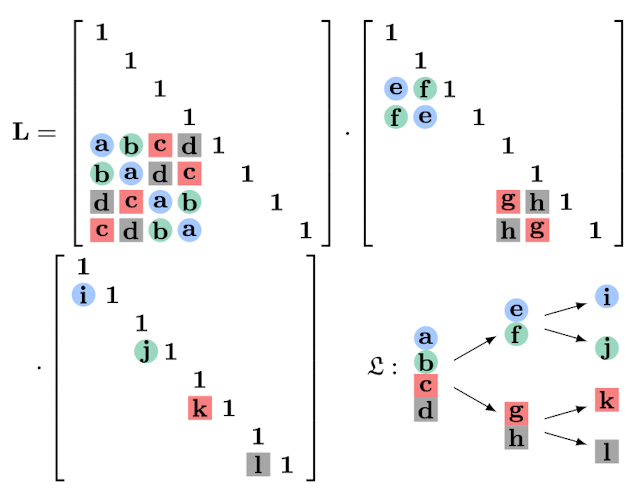
\includegraphics[width=0.5\textwidth]{Figure/LDL_example.png}
	\caption{The factorization tree $\mathbf{L}_2, \mathbf{L}_1, \mathbf{L}_0, \tilde{\mathbf{B}}_0$ for $d=8$, from~\cite{DP16}.}
	\label{fig:dp16-tree}
\end{figure}

\begin{proof}
	We proceed by induction on $d$. When $d$ is prime this is the regular GSO. Suppose $d$ is composite and the claim holds for all $R_{d'}$ with $d' < d$.

	By the properties above, $\mathbf{B}_{h-1} := M_{d/d_{h-1}}(\mathbf{b})$ is full-rank, so it decomposes as $\mathbf{B}_{h-1} = \mathbf{L}_{h-1} \tilde{\mathbf{B}}$, where $\mathbf{L}_{h-1} \in R_{d_{h-1}}^{d/d_{h-1} \times d/d_{h-1}}$ is unit lower-triangular and $\tilde{\mathbf{B}} \in R_{d_{h-1}}^{d/d_{h-1} \times md/d_{h-1}}$ is orthogonal. Write $\tilde{\mathbf{B}} = [\mathbf{b}_1, \dots, \mathbf{b}_{d/d_{h-1}}]$ as row vectors in $R_{d_{h-1}}^{md/d_{h-1}}$. By the induction hypothesis, each decomposes as
	\[
		M_{d_{h-1}/1}(\mathbf{b}_j) = \left( \prod_{i=0}^{h-2} M_{d_i/1}(\mathbf{L}_{i,j}) \right) \cdot \tilde{\mathbf{B}}_j \qquad \forall j \in [d/d_{h-1}],
	\]
	where $\tilde{\mathbf{B}}_j \in \R^{d_{h-1} \times md}$ is orthogonal and $\mathbf{L}_{i,j} \in R_{d_i}^{(d_{h-1}/d_i) \times (d_{h-1}/d_i)}$ is block-diagonal with $d_{h-1}/d_{i+1}$ diagonal blocks in $R_{d_i}^{(d_{i+1}/d_i) \times (d_{i+1}/d_i)}$.

	Therefore,
	\begin{align*}
		M_{d/1}(\mathbf{b}) &= M_{d_{h-1}/1}(M_{d/d_{h-1}}(\mathbf{b})) = M_{d_{h-1}/1}(\mathbf{B}_{h-1}) \\
		&= M_{d_{h-1}/1}(\mathbf{L}_{h-1}) \cdot M_{d_{h-1}/1}(\tilde{\mathbf{B}}) \\
		&= M_{d_{h-1}/1}(\mathbf{L}_{h-1}) \cdot [M_{d_{h-1}/1}(\mathbf{b}_1), \dots, M_{d_{h-1}/1}(\mathbf{b}_{d/d_{h-1}})] \\
		&= M_{d_{h-1}/1}(\mathbf{L}_{h-1}) \cdot \left[ \left( \prod_{i=0}^{h-2} M_{d_i/1}(\mathbf{L}_{i,j}) \right) \cdot \tilde{\mathbf{B}}_j \right]_{j \in [d/d_{h-1}]}.
	\end{align*}
	Let $\mathbb{L}_{i,j} := M_{d_i/1}(\mathbf{L}_{i,j}) \in \R^{d_{h-1} \times d_{h-1}}$ and $\tilde{\mathbf{B}}_0 := [\tilde{\mathbf{B}}_1, \dots, \tilde{\mathbf{B}}_{d/d_{h-1}}]$. Then
	\[
		M_{d/1}(\mathbf{b}) = M_{d_{h-1}/1}(\mathbf{L}_{h-1}) \cdot \left( \prod_{i=0}^{h-2} \mathrm{Diag}(\{\mathbb{L}_{i,j}\}_j) \right) \cdot \tilde{\mathbf{B}}_0,
	\]
	where
	\[
		\mathrm{Diag}(\{\mathbb{L}_{i,j}\}_j) = \begin{bmatrix}
			\mathbb{L}_{i,1} & 0 & \cdots & 0 \\
			0 & \mathbb{L}_{i,2} & \cdots & 0 \\
			\ddots & \ddots & \ddots & \ddots \\
			0 & 0 & \cdots & \mathbb{L}_{i,d/d_{h-1}}
		\end{bmatrix}.
	\]
	Setting
	\[
		\mathbf{L}_i := \mathrm{Diag}(\{\mathbf{L}_{i,j}\}_j) = \begin{bmatrix}
			\mathbf{L}_{i,1} & 0 & \cdots & 0 \\
			0 & \mathbf{L}_{i,2} & \cdots & 0 \\
			\ddots & \ddots & \ddots & \ddots \\
			0 & 0 & \cdots & \mathbf{L}_{i,d/d_{h-1}}
		\end{bmatrix},
	\]
	we have $\mathrm{Diag}(\{\mathbb{L}_{i,j}\}_j) = M_{d_i/1}(\mathbf{L}_i)$, so
	\[
		M_{d/1}(\mathbf{b}) = M_{d_{h-1}/1}(\mathbf{L}_{h-1}) \cdot \left( \prod_{i=0}^{h-2} M_{d_i/1}(\mathbf{L}_i) \right) \cdot \tilde{\mathbf{B}}_0 = \left( \prod_{i=0}^{h-1} M_{d_i/1}(\mathbf{L}_i) \right) \cdot \tilde{\mathbf{B}}_0.
	\]

	Finally we check the requirements. $\mathbf{L}_i$ has $d/d_{h-1}$ blocks in $R_{d_i}^{(d_{h-1}/d_i) \times (d_{h-1}/d_i)}$, each with $d_{h-1}/d_{i+1}$ blocks in $R_{d_i}^{(d_{i+1}/d_i) \times (d_{i+1}/d_i)}$, hence $d/d_{i+1}$ such blocks overall, as required.

	For orthogonality of $\tilde{\mathbf{B}}_0 = [\tilde{\mathbf{B}}_1, \dots, \tilde{\mathbf{B}}_{d/d_{h-1}}]$: two row vectors $\mathbf{u}, \mathbf{v}$ within the same $\tilde{\mathbf{B}}_j$ are orthogonal by the induction hypothesis. If $\mathbf{u}$ belongs to $\tilde{\mathbf{B}}_j$ and $\mathbf{v}$ to $\tilde{\mathbf{B}}_\ell$ ($j \ne \ell$), write $\mathbf{u} = \mathbf{a}_j \cdot M_{d_{h-1}/1}(\mathbf{b}_j)$ and $\mathbf{v} = \mathbf{a}_\ell \cdot M_{d_{h-1}/1}(\mathbf{b}_\ell)$ for some $\mathbf{a}_j, \mathbf{a}_\ell \in \R^{d_{h-1}}$, and let $a_j = V_{d_{h-1}/1}^{-1}(\mathbf{a}_j)$, $a_\ell = V_{d_{h-1}/1}^{-1}(\mathbf{a}_\ell)$. By the properties above,
	\begin{align*}
		\langle \mathbf{u}, \mathbf{v} \rangle_2
		&= \langle \mathbf{a}_j \cdot M_{d_{h-1}/1}(\mathbf{b}_j), \mathbf{a}_\ell \cdot M_{d_{h-1}/1}(\mathbf{b}_\ell) \rangle_2 \\
		&= \langle V_{d_{h-1}/1}(a_j) \cdot M_{d_{h-1}/1}(\mathbf{b}_j), V_{d_{h-1}/1}(a_\ell) \cdot M_{d_{h-1}/1}(\mathbf{b}_\ell) \rangle_2 \\
		&= \langle V_{d_{h-1}/1}(a_j \cdot \mathbf{b}_j), V_{d_{h-1}/1}(a_\ell \cdot \mathbf{b}_\ell) \rangle_2 \\
		&= \langle a_j \cdot \mathbf{b}_j, a_\ell \cdot \mathbf{b}_\ell \rangle_2 = 0.
	\end{align*}
\end{proof}

\subsection{LDL Decomposition in \texorpdfstring{$R_d^{n \times m}$}{Rd\^{}(n x m)}}

\begin{theorem}
	\label{thm:ldl-rdnm}
	Let $1 = d_0 \mid d_1 \mid \dots \mid d_h = d$ be a tower of proper divisors of $d$, and let $\mathbf{B} \in R_d^{n \times m}$ be full-rank. Then there is a GSO of $M_{d/1}(\mathbf{B})$
	\[
		M_{d/1}(\mathbf{B}) = \left( \prod_{i=0}^{h} M_{d_i/1}(\mathbf{L}_i) \right) \cdot \tilde{\mathbf{B}}_0 = \mathbf{L} \cdot \tilde{\mathbf{B}}_0,
	\]
	where $\tilde{\mathbf{B}}_0 \in \R^{nd \times md}$ is orthogonal and $\mathbf{L}_i \in R_{d_i}^{(n(d/d_i)) \times (n(d/d_i))}$ is block-diagonal, each block a unit lower-triangular matrix of $R_{d_i}^{(d_{i+1}/d_i) \times (d_{i+1}/d_i)}$, with $n(d/d_{i+1})$ diagonal blocks. Moreover, the LDL decomposition of $M_{d/1}(\mathbf{BB}^*)$ is $\mathbf{L} \cdot (\tilde{\mathbf{B}}_0 \tilde{\mathbf{B}}_0^t) \cdot \mathbf{L}^t$.
\end{theorem}

\begin{proof}
	Let $\mathbf{B} = \mathbf{L}_h \mathbf{B}'$, where $\mathbf{L}_h$ is unit lower-triangular and $\mathbf{B}' = [\mathbf{b}_1', \dots, \mathbf{b}_n']$ is orthogonal. Applying Theorem~\ref{thm:ldl-rdm} to each $\mathbf{b}_j'$ gives
	\[
		M_{d/1}(\mathbf{b}_j') = \left( \prod_{i=0}^{h-1} M_{d_i/1}(\mathbf{L}_{i,j}) \right) \cdot \tilde{\mathbf{B}}_j \qquad \forall j \in [n].
	\]
	Setting $\tilde{\mathbf{B}}_0 = [\tilde{\mathbf{B}}_1, \dots, \tilde{\mathbf{B}}_n]$ and $\mathbf{L}_i = \mathrm{Diag}(\{\mathbf{L}_{i,j}\}_j)$,
	\begin{align*}
		M_{d/1}(\mathbf{B})
		&= M_{d/1}(\mathbf{L}_h) \cdot M_{d/1}([\mathbf{b}_1', \dots, \mathbf{b}_n']) \\
		&= M_{d/1}(\mathbf{L}_h) \cdot [M_{d/1}(\mathbf{b}_1'), \dots, M_{d/1}(\mathbf{b}_n')] \\
		&= M_{d/1}(\mathbf{L}_h) \cdot \left[ \left( \prod_{i=0}^{h-1} M_{d_i/1}(\mathbf{L}_{i,j}) \right) \cdot \tilde{\mathbf{B}}_j \right]_{j \in [n]} \\
		&= M_{d/1}(\mathbf{L}_h) \cdot \left( \prod_{i=0}^{h-1} M_{d_i/1}(\mathbf{L}_i) \right) \cdot \tilde{\mathbf{B}}_0 \\
		&= \left( \prod_{i=0}^{h} M_{d_i/1}(\mathbf{L}_i) \right) \cdot \tilde{\mathbf{B}}_0.
	\end{align*}
\end{proof}

This shows that for any full-rank $\mathbf{B} \in R_d^{n \times m}$, the GSO of $M_{d/1}(\mathbf{B})$ — equivalently the LDL decomposition of $M_{d/1}(\mathbf{BB}^*)$ — factors, with each $\mathbf{L}_i$ a unit lower-triangular, sparse, block-diagonal matrix.

\subsection{Decomposition Algorithm}

Since $V_{d/d'}$ and $M_{d/d'}$ compute efficiently in FFT form, we obtain the fast Fourier GSO algorithm.

\begin{algorithm}[H]
	\caption{$\mathsf{ffGSO}(\mathbf{B} \in R_d^{n \times m})$}
	\label{alg:ffgso}
	\begin{algorithmic}[1]
		\Require $\mathbf{B} \in R_d^{n \times m}$
		\Ensure Factorization tree $(\mathbf{L}, (\mathfrak{L}_i)_i)$
		\State $(\mathbf{L}, \mathbf{B}') \gets \mathsf{GSO}_{R_d}(\mathbf{B})$
		\If{$d = 1$}
			\State \Return $(\mathbf{L}, \mathbf{B}')$
		\EndIf
		\State Let $\mathbf{B}' = [\mathbf{b}_1', \dots, \mathbf{b}_n']$
		\State $d' \gets \mathrm{gpd}(d)$
		\For{$i = 1$ to $n$}
			\State $\mathfrak{L}_i \gets \mathsf{ffGSO}_{R_{d'}}(M_{d/d'}(\mathbf{b}_i'))$
		\EndFor
		\State \Return $\mathbf{L}, (\mathfrak{L}_i)_{1 \leq i \leq n}$
	\end{algorithmic}
\end{algorithm}

In practice we favor LDL over GSO, since it lets us ignore the row-vector length $m$, gaining a factor of $\Theta(m)$.

\begin{algorithm}[H]
	\caption{$\mathsf{ffLDL}(\mathbf{G} \in R_d^{n \times n})$}
	\label{alg:ffldl}
	\begin{algorithmic}[1]
		\Require $\mathbf{G} \in R_d^{n \times n}$
		\Ensure Factorization tree $(\mathbf{L}, (\mathfrak{L}_i)_i)$
		\State Transform $\mathbf{G}$ into FFT domain if it is not already
		\State $(\mathbf{L}, \mathbf{D}) \gets \mathsf{LDL}_{R_d}(\mathbf{G})$
		\If{$d = 1$}
			\State \Return $(\mathbf{L}, \mathbf{D})$
		\EndIf
		\State $d' \gets \mathrm{gpd}(d)$
		\For{$i = 1$ to $n$}
			\State $\mathfrak{L}_i \gets \mathsf{ffLDL}_{R_{d'}}(M_{d/d'}(\mathbf{D}_{ii}))$
		\EndFor
		\State \Return $\mathbf{L}, (\mathfrak{L}_i)_{1 \leq i \leq n}$
	\end{algorithmic}
\end{algorithm}

Note that $\mathbf{D}_{ii} = \mathbf{b}_i' \mathbf{b}_i'^*$, as in $\mathsf{ffGSO}$.

\subsubsection{Complexity}

Let $C(n,d)$ be the complexity of $\mathsf{ffLDL}(\mathbf{G} \in R_d^{n \times n})$. Then
\[
	C(n,d) = \Theta(n^2 d \log d) + \Theta(n^3 d) + \Theta(d(d/d_{h-1})^2) + n \, C(d/d_{h-1}, d_{h-1}),
\]
where the first term is the FFT of the $n^2$ coefficients of $\mathbf{G}$ (absent in recursive calls, already in FFT form); the second is $\mathsf{LDL}_{R_d}(\mathbf{G})$ in FFT form ($n^3$ multiplications in $R_d$, each costing $\Theta(d)$); the third is computing $M_{d/d_{h-1}}(\mathbf{D}_{ii})$; and the last is the $n$ recursive calls.

Let $k_h = d_h/d_{h-1}$. Expanding the recursion,
\begin{align*}
	C(k_h, d_{h-1}) &= \sum_{i=1}^h \frac{d}{d_i} \Theta(k_i^3 d_{i-1}) + \sum_{i=1}^h \frac{d}{d_i} \Theta(d_{i-1} k_i^2) + \frac{d}{d_1} C(k_1, 1) \\
	&= \sum_{i=1}^h \frac{d}{d_i} \Theta(k_i^3 d_{i-1}) = \sum_{i=1}^h \frac{d}{d_i} \Theta\!\left( \left( \frac{d_i}{d_{i-1}} \right)^3 d_{i-1} \right) = \Theta(d) \sum_{i=1}^h k_i^2.
\end{align*}
Hence
\[
	C(n,d) = \Theta(n^2 d \log d) + \Theta(n^3 d) + \Theta(nd) \sum_{i=1}^h k_i^2.
\]

\subsection{Fast Fourier Nearest-Plane \texorpdfstring{$\mathsf{ffNP}_{R_d}(\mathbf{t}, \mathfrak{L})$}{ffNP\_Rd(t,L)}}

Let $Z_d = \Z[X]/(X^d - 1)$. The $\mathsf{ffNP}$ algorithm takes a target $\mathbf{t} \in R_d^n$ and a precomputed decomposition tree $\mathfrak{L} \gets \mathsf{ffLDL}(\mathbf{BB}^*)$.

\begin{algorithm}[H]
	\caption{$\mathsf{ffNP}_{R_d}(\mathbf{t}, \mathfrak{L})$}
	\label{alg:ffnp}
	\begin{algorithmic}[1]
		\Require $\mathbf{t} \in R_d^n$, factorization tree $\mathfrak{L}$
		\Ensure $\mathbf{z} \in Z_d^n$
		\If{$d = 1$}
			\State $(\mathbf{L}, \mathbf{D}) \gets \mathfrak{L}$
			\State \Return $\mathsf{NP}_\R(\mathbf{t}, \mathbf{L})$
		\EndIf
		\State $(\mathbf{L}, (\mathfrak{L}_i)_{1 \leq i \leq n}) \gets \mathfrak{L}$
		\State $d' \gets \mathrm{gpd}(d)$
		\For{$j = n$ to $1$}
			\State $\overline{\mathbf{t}_j} \gets \mathbf{t}_j + \sum_{i>j} (\mathbf{t}_i - \mathbf{z}_i) \mathbf{L}_{ij}$
			\State $\mathbf{z}_j \gets V_{d/d'}^{-1}\!\left( \mathsf{ffNP}_{R_{d'}}(V_{d/d'}(\overline{\mathbf{t}_j}), \mathfrak{L}_j) \right)$
		\EndFor
		\State \Return $\mathbf{z} = (\mathbf{z}_1, \dots, \mathbf{z}_n)$
	\end{algorithmic}
\end{algorithm}

\begin{lemma}
	\label{lem:ffnp}
	For $\mathbf{B} = [\mathbf{b}_1, \dots, \mathbf{b}_n] \in R_d^{n \times m}$ and its GSO $\tilde{\mathbf{B}} = [\tilde{\mathbf{b}}_1, \dots, \tilde{\mathbf{b}}_n]$ in $R_d$,
	\[
		(\mathbf{z} - \mathbf{t}) \cdot \mathbf{B} = (\mathbf{z} - \overline{\mathbf{t}}) \cdot \tilde{\mathbf{B}}.
	\]
\end{lemma}

\begin{proof}
	Recall $\tilde{\mathbf{b}}_i = \mathbf{b}_i - \sum_{j<i} \mathbf{L}_{ij} \tilde{\mathbf{b}}_j$. Then
	\begin{align*}
		(\mathbf{z} - \overline{\mathbf{t}}) \cdot \tilde{\mathbf{B}}
		&= \sum_{j=1}^n (\mathbf{z}_j - \overline{\mathbf{t}}_j) \cdot \tilde{\mathbf{b}}_j \\
		&= \sum_{j=1}^n \left[ \mathbf{z}_j - \left( \mathbf{t}_j + \sum_{i>j} (\mathbf{t}_i - \mathbf{z}_i) \mathbf{L}_{ij} \right) \right] \cdot \tilde{\mathbf{b}}_j \\
		&= \sum_{j=1}^n \left[ (\mathbf{z}_j - \mathbf{t}_j) + \sum_{i>j} (\mathbf{z}_i - \mathbf{t}_i) \mathbf{L}_{ij} \right] \cdot \tilde{\mathbf{b}}_j \\
		&= \sum_{j=1}^n \left[ \sum_{i \geq j} (\mathbf{z}_i - \mathbf{t}_i) \mathbf{L}_{ij} \right] \cdot \tilde{\mathbf{b}}_j \\
		&= \sum_{i=1}^n (\mathbf{z}_i - \mathbf{t}_i) \cdot \sum_{j \leq i} \mathbf{L}_{ij} \cdot \tilde{\mathbf{b}}_j \\
		&= \sum_{i=1}^n (\mathbf{z}_i - \mathbf{t}_i) \cdot \mathbf{b}_i \\
		&= (\mathbf{z} - \mathbf{t}) \cdot \mathbf{B}.
	\end{align*}
\end{proof}

\begin{remark}
	If we instead apply $\mathsf{NP}_\R$ directly to $c(\mathbf{t}) \in \R^{nd}$, then by the results of the previous section $(c(\mathbf{z}) - c(\mathbf{t})) \cdot C(\mathbf{B}) = (c(\mathbf{z}) - c(\mathbf{t}')) \cdot C(\tilde{\mathbf{B}})$ for some $\mathbf{t}'$. Lemma~\ref{lem:ffnp} shows $(c(\mathbf{z}) - c(\mathbf{t})) \cdot C(\mathbf{B}) = (c(\mathbf{z}) - c(\overline{\mathbf{t}})) \cdot C(\tilde{\mathbf{B}})$, so $c(\mathbf{t}') = c(\overline{\mathbf{t}})$: running $\mathsf{NP}_\R$ on $c(\mathbf{t})$ and $C(\mathbf{B}), C(\tilde{\mathbf{B}})$ computes exactly what $\mathsf{ffNP}_{R_d}$ computes — just faster.

	The complexity of $\mathsf{NP}_\R$ on $c(\mathbf{t}) \in \R^{nd}$ is $\Theta((nd)^2)$, while $\mathsf{ffNP}_{R_d}$ on $\mathbf{t} \in R_d^n$ costs $\Theta(n^2 d) + \Theta(nd) \sum_{i=1}^h k_i^2$. For Falcon-512 ($n=2$, $d=512$): $1024^2$ versus $2048 + 1024 \cdot \sum_{i=1}^9 2 = 2048 + 1024 \cdot 18$.
\end{remark}

\begin{theorem}
	\label{thm:ffnp-guarantee}
	Let $\tilde{\mathbf{B}}_0$ be the orthogonalization of $M_{d/1}(\mathbf{B})$ over $\R$. Then
	\[
		V_{d/1}((\mathbf{z} - \mathbf{t})\mathbf{B}) \in \mathcal{P}(\tilde{\mathbf{B}}_0) = \left[-\frac{1}{2}, \frac{1}{2}\right]^n \cdot \tilde{\mathbf{B}}_0.
	\]
\end{theorem}

\begin{proof}
	For $d = 1$ this is exactly the guarantee of $\mathsf{NP}_\R(\mathbf{t}, \mathbf{L})$. Assume the claim for all $d' < d$, and let $d' = \mathrm{gpd}(d)$.

	By construction $\mathfrak{L}_j = \mathsf{ffGSO}_{R_{d'}}(M_{d/d'}(\mathbf{b}_j'))$, where $\mathbf{B} = \mathbf{L} \cdot [\mathbf{b}_1', \dots, \mathbf{b}_n']$, and $V_{d/d'}(\mathbf{z}_j) = \mathsf{ffNP}_{R_{d'}}(V_{d/d'}(\overline{\mathbf{t}_j}), \mathfrak{L}_j)$. Writing $\mathbf{B}_j' = M_{d/d'}(\mathbf{b}_j')$ and letting $\tilde{\mathbf{B}}_j$ be the orthogonalization of $M_{d'/1}(\mathbf{B}_j') = M_{d/1}(\mathbf{b}_j')$, the induction hypothesis gives
	\[
		V_{d'/1}\big( (V_{d/d'}(\mathbf{z}_j) - V_{d/d'}(\mathbf{t}_j)) \cdot \mathbf{B}_j' \big) \in \mathcal{P}(\tilde{\mathbf{B}}_j),
	\]
	equivalently
	\[
		V_{d/1}((\mathbf{z}_j - \mathbf{t}_j) \cdot \mathbf{b}_j') \in \mathcal{P}(\tilde{\mathbf{B}}_j).
	\]
	By Lemma~\ref{lem:ffnp}, $(\mathbf{z} - \mathbf{t}) \cdot \mathbf{B} = \sum_{j=1}^n (\mathbf{z}_j - \overline{\mathbf{t}}_j) \cdot \mathbf{b}_j'$, so
	\[
		V_{d/1}((\mathbf{z} - \mathbf{t}) \cdot \mathbf{B}) \in \mathcal{P}([\tilde{\mathbf{B}}_1, \dots, \tilde{\mathbf{B}}_n]).
	\]
	By Theorem~\ref{thm:ldl-rdnm}, $[\tilde{\mathbf{B}}_1, \dots, \tilde{\mathbf{B}}_n] = \tilde{\mathbf{B}}_0$ is the orthogonalization of $M_{d/1}(\mathbf{B})$, completing the proof.

\end{proof}

\subsubsection{Complexity}

Let $C(n,d)$ be the complexity of $\mathsf{ffNP}_{R_d}(\mathbf{t}, \mathfrak{L})$ for $\mathbf{t} \in R_d^n$. Then, with $1 = d_0 \mid d_1 \mid \dots \mid d_h = d$ a tower of divisors and $k_h = d_h/d_{h-1}$,
\[
	C(n,d) = \Theta(nd \log d) + \Theta(n^2 d) + \Theta(nd k_h^2) + n \, C(k_h, d_{h-1}),
\]
where the first term is the FFT of the $n$ coefficients of $\mathbf{t}$; the second is the $n$ updates $\overline{\mathbf{t}_j} \gets \mathbf{t}_j + \sum_{i>j}(\mathbf{t}_i - \mathbf{z}_i)\mathbf{L}_{ij}$ in FFT form; the third is computing $V_{d/\mathrm{gpd}(d)}$ and its inverse; and the last is the recursive calls. Expanding the recursion and dropping the (dominated) first term,
\[
	C(k_h, d_{h-1}) = \sum_{1 \leq i \leq h} \frac{d}{d_i} \Theta(d_{i-1} k_i^3) + \frac{d}{d_1} C(k_1, d_0) = \Theta(d) \sum_{i=1}^h k_i^2,
\]
so
\[
	C(n,d) = \Theta(nd \log d) + \Theta(n^2 d) + \Theta(nd) \sum_{i=1}^h k_i^2.
\]

\subsection{Application in the Cyclotomic Ring \texorpdfstring{$F_d$}{Fd}}

All of the above transfers from $R_d = \R[X]/(X^d-1)$ to the cyclotomic ring $F_d$:
\begin{itemize}
	\item $\xi_d = e^{2\pi i/d}$, $\Omega_d = \{\xi_d^k \mid k \in \Z_d, \gcd(k,d)=1\}$.
	\item $\phi_d(X) = \prod_{\xi \in \Omega_d} (X - \xi) = \prod_{k \in \Z_d^\times} (X - \xi_d^k)$.
	\item $\psi_d(X) = \prod_{\xi^d=1,\, \xi \notin \Omega_d} (X - \xi) = \prod_{k \in \Z_d \setminus \Z_d^\times} (X - \xi_d^k)$.
	\item $\deg(\phi_d) = \varphi(d)$, the Euler totient function of $d$.
	\item $\phi_d(X) \psi_d(X) = X^d - 1$.
	\item $F_d = \R[X]/(\phi_d(X))$.
	\item When $d = 2^n$, $\phi_d(X) = X^{d/2} + 1$.
\end{itemize}

\begin{definition}
	Let $e_d$ be the unique element of $R_d$ such that
	\[
		e_d = \begin{cases} 1 \bmod \phi_d \\ 0 \bmod \psi_d. \end{cases}
	\]
	Define the embedding $\iota_d : F_d \to R_d$ by $\iota_d(f) = f \cdot e_d$, equivalently
	\[
		\iota_d(f)(\xi) = \begin{cases} f(\xi) & \text{if } \phi_d(\xi) = 0, \\ 0 & \text{if } \psi_d(\xi) = 0. \end{cases}
	\]
	With $\iota_d$, define the linear maps
	\[
		V_{d/d'}' := \iota_{d'}^{-1} \circ V_{d/d'} \circ \iota_d, \qquad M_{d/d'}' := \iota_{d'}^{-1} \circ M_{d/d'} \circ \iota_d.
	\]
\end{definition}


%-------------------
%% Reference List
\pagebreak

\nocite{*}
\printbibliography

\end{document}
